\chapter{Detector Design and Construction Organization}
\label{vl:tc-overview}

\Dword{tc} is led by the \dword{tcoord}, who runs the \dword{tb} that
reviews \dword{dune} technical options. The \dword{tc} organizational
chart is shown in Fig.~\ref{fig:TC_org_chart}.
\begin{dunefigure}[\dword{tc} organizational chart]{fig:TC_org_chart}
  {\dword{dune} \dword{tc} organizational chart.}
  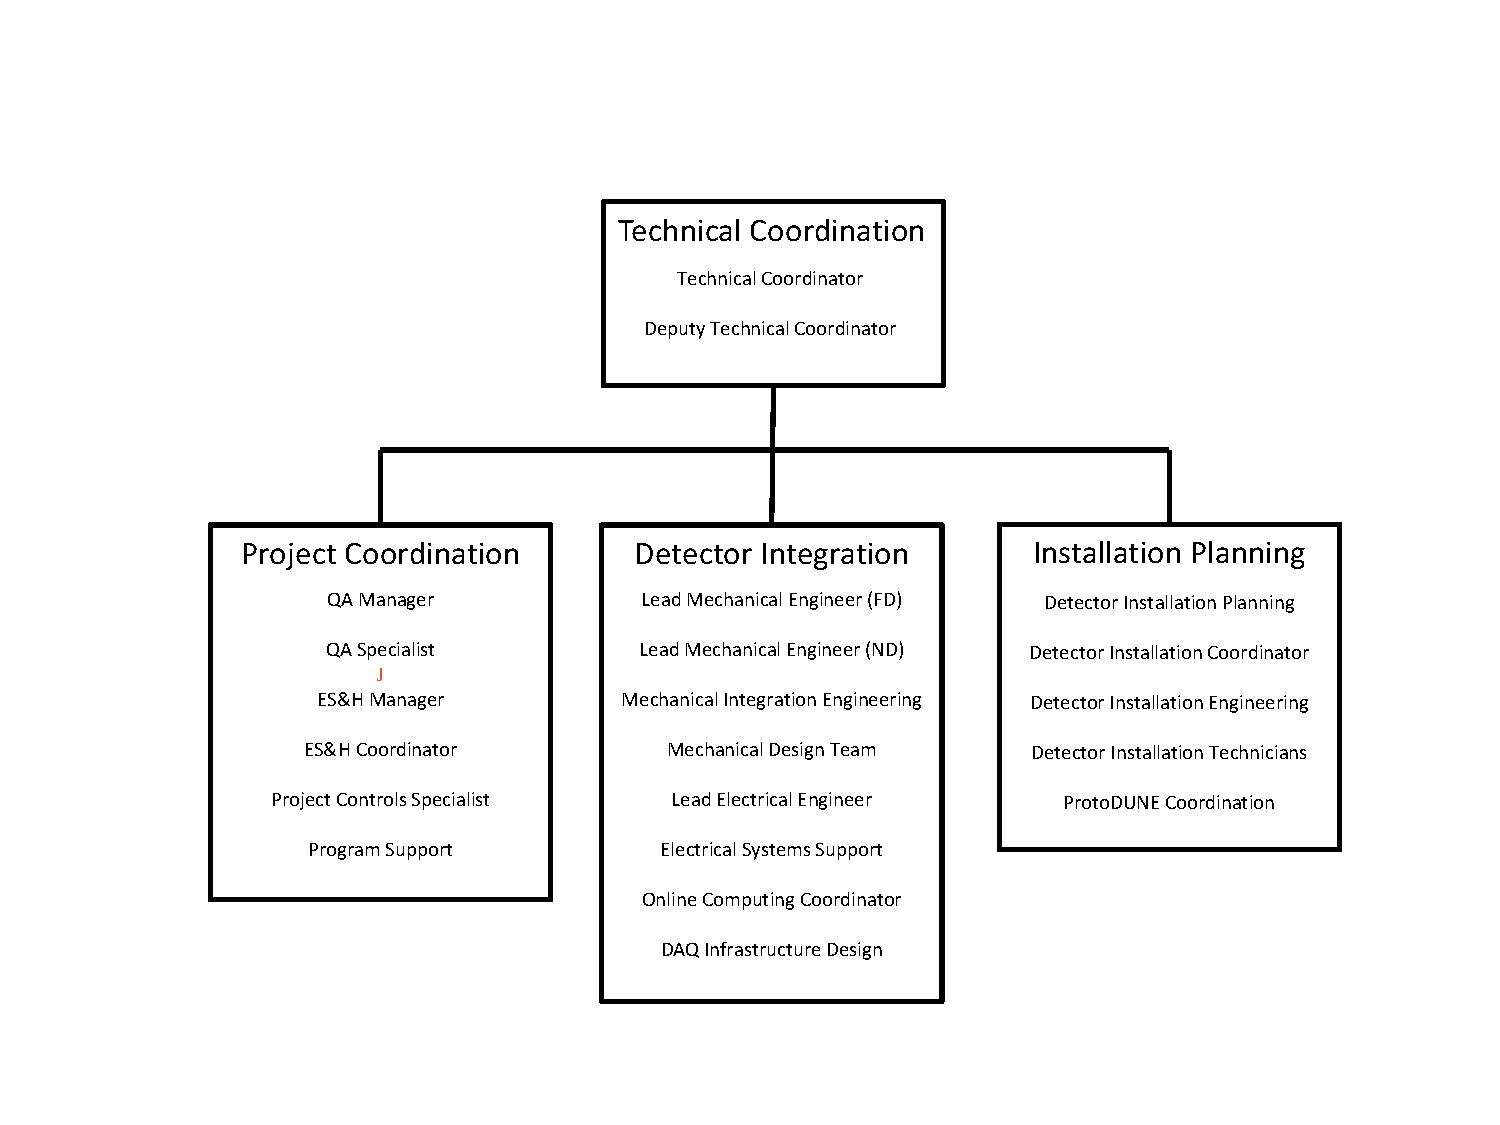
\includegraphics[width=0.99\textwidth]{TC_org_chart}
\end{dunefigure}


\section{DUNE Far Detector Consortia}
\label{sec:consortia}

Construction of the \dword{dune} far \dwords{detmodule} is carried out by
``consortia of collaboration institutions'' who assume responsibility
for detector subsystems.  Each consortium plans and
executes the construction, installation and commissioning of its 
subsystem.

A total of eleven \dword{fd} consortia have been formed to cover the
subsystems required for the two \dword{lartpc} designs, \dword{sp} and
\dword{dp}, currently under consideration.  Three consortia pursue
subsystems specific to the \dword{sp} design (\dword{apa}, \dword{ce},
and \dword{pds}) and another three consortia pursue designs for
\dword{dp} specific subsystems (\dword{crp}, TPC electronics and a
\dword{dp} \dword{pds}).  An additional five consortia are responsible
for subsystems common to both detector technologies; these are
\dword{hv}, \dword{daq}, \dword{cisc}, calibration and computing.

A consortium leader and a technical lead manage each consortium.  The
consortium leader chairs an institutional board composed of one
representative from each of the contributing institutions.
Significant consortium decisions, such as technology selections and
assignment of responsibilities among the institutions, are first
passed through this board, then passed as recommendations to the
\dword{dune} \dword{exb} for formal collaboration approval.

In many cases, multiple institutions within a consortium, potentially
supported by different funding agencies, share responsibility for a
particular subsystem deliverable.  \dword{dune} expects each
participating funding agency to manage its own internal project
responsibilities.  The consortium technical lead coordinates the
separate internal projects. This person also chairs a consortium
project management board, composed of the managers of each internal
project, that oversees the interconnections between the different
efforts.

%\section{(suggested) Executive Board}

The \dword{dune} \dword{exb} is the primary collaboration
decision-making body and as such includes representatives from all
major areas of activity within the collaboration.  All collaboration
decisions, especially those with potential impact on the \dword{dune}
scientific program or connected with the assignment of institutional
responsibilities, pass through the \dword{exb}.  \dword{exb} decisions
are expected to be achieved through consensus.  In cases where
consensus cannot be obtained, decision-making responsibility passes to
the co-spokespersons. The consortium leader represents the consortium
on the \dword{exb}.

\section{Technical Coordination (TCN)}
\label{sec:tc}

Because the consortia operate as self-managed entities, a strong
\dword{tc} organization is required to ensure overall integration of
the detector elements and successful execution of the detector
construction project.  \dword{tc} responsibility includes project
oversight, systems engineering, quality assurance, and safety.
\dword{tc} provides support to the \dword{jpo} (see
Section~\ref{sec:pm}) for planning and executing the required detector
integration and installation activities in the nearby surface
facilities and underground detector caverns at \surf.

\dword{tc} is headed by the \dword{tcoord}, who is an \dword{fnal}
employee and is appointed jointly by the \dword{fnal} director and the
\dword{dune} co-spokespersons.  A deputy technical coordinator is
selected from within the collaboration to assist the \dword{tc}.

The \dword{tc} organization supports the work of the consortia and
takes responsibility for integration of the detector
subsystems.  The organization includes teams focused on project
coordination, detector integration, and installation support.  The
project coordination team is led by a lead project controls
specialist, a \dword{qa} manager, and an \dword{esh} manager.  The
detector integration team is directed by a lead mechanical and lead
electrical engineer, and includes an online computing coordinator.
The installation support team is headed by the coordinators for
activities associated with the integration of detector components on
the surface and installation of components in the underground areas.
Each of the three teams incorporates additional personnel that support
these individuals in carrying out their areas of responsibility.

\section{DUNE Project Management}
\label{sec:pm}

\fixme{I'm not clear on the distinction between board meetings:
  consortium board meetings with all consortium leads? Then tech board
  meetings are at a higher level? Who is involved? Then PMBs with
  funding agencies (since they are responsible for managing their
  projects?}

The \dword{tcoord} manages the overall detector construction project
through regular Technical Board meetings with the consortia leadership
teams and members of the \dword{tc} organization.  These board
meetings provide the primary forums for required interactions between
the consortia leadership teams.

Technical Board meetings are used to evaluate consortia design
decisions with potential impacts on overall detector performance,
ensure that interfaces between the different subsystems are well
understood and documented, and monitor the overall construction
project to identify and address both technical and interface issues as
they arise.

Project board meetings are used to ensure that the scopes of each
consortium are fully documented with assigned institutional
responsibilities, develop and manage risks held within a global
project registry, review and manage project change requests, and
monitor the status of the overall detector construction schedule.

Any decisions generated through these board meetings are passed to the
\dword{dune} \dword{exb} as recommendations for formal approval.
Depending on the specific agenda items for a meeting, the
\dword{tcoord} will invite additional members of the collaboration
with specific knowledge or particular expertise to participate.  In
addition, for major decisions, the \dword{tcoord} will officially
appoint three internal collaboration referees with no direct conflicts
of interest to engage in the process.

\section{Technical Coordination (TCN) Resources}
\label{sec:tc_resources}

Resources for the personnel and activities associated with \dword{tc}
are provided through a mixture of common collaboration funds and
support from the host nation.  During the construction phase of the
experiment, \dword{dune} will collect an annual membership fee from
each institution based on the number of Ph.D scientists contributing
to the collaboration.  The collected funds will be used primarily for
supporting the personnel on the \dword{tc} team.  Funding agencies
will have the option of directly providing team members in lieu of
monetary contributions.

The acquisition of common infrastructure will be supported through
additional collaboration common funds collected from the funding
agencies as a percentage of the value of their contributed detector
deliverables.  As in the case above, \dword{dune} will give funding
agencies the option of directly providing equivalently valued
infrastructure items as opposed to monetary contributions.  Host
laboratory functions provided by the SDSD will be supported directly
by the host nation funding agency, DOE.

All project partners will sign \dwords{mou} that specify which
detector deliverables each supporting funding will provide. The
\dword{mou} will also specify the required common fund contributions
from each participating funding agency.  The \dword{dune} resource
coordinator will be responsible for managing and reporting on all
common fund contributions.

%%%%%%%%%%%%%%%%%%%%%%%%%%%%%%%%
\section{ProtoDUNE-2}
\label{sec:fdsp-coord-protodune2}

%%%%%%%%%%%%%%%%%%%%%%%%%%%%%%%%
\section{Interface to National Projects}
\label{sec:fdsp-coord-national}

\dword{dune} \dword{tc} works with each consortium leadership
team. The consortia leadership teams comprise the consortia leaders
and consortia technical leaders as well as others appointed by the
consortia leaders. The consortia leadership teams usually have
representatives from the various national projects that provide the
funding to build the consortia deliverables. If the consortia
leadership teams are not directly embedded in the various national
projects building their subsystem, then the consortia leadership teams
must still represent their national projects to \dword{tc}. The
consortia leadership teams are responsible for providing their
deliverables on time according to the \dword{ims}. They are
responsible for identifying any inconsistencies between the
\dword{ims} and their national project schedules and bringing these
issues to \dword{tc}. The consortia leadership teams are responsible
for reporting progress against the \dword{ims} to \dword{tc}.
